\newpage
\section{Prinsipiell løsning}
\label{prinsipiellLoesning}

\subsection{Hvit støy}
\label{hvitStoeoy}
Hvit støy er et signal som er helt flatt på spektrums analysen og har en konstant effekt over alle frekvenser. For å kunne generere hvit støy trenger man en pseudo tilfeldig algoritme som kan tilfelig velge hvilken frekvens som sendes ut av FPGAen. Det kan løses ved å implementere LFSR (Linear Feedback Shift Register) som er en algoritme som genererer en pseudo tilfeldig sekvens av bits. LFSR er en algoritme som er lett å implementere i hardware og er derfor mye brukt i FPGAer. LFSR er en algoritme som bruker XOR operasjoner for å generere en pseudo tilfeldig sekvens av bits ved en høy frekvens. Ettersom bitsene kommer ut i en tilfeldig rekkefølge vil frekvenskomponentene sin styrke i signalet være jevnt fordelt. LFSR implementeres ved å sette mange D-vipper etterhverandre og kobinere noen utganger i en XOR som vist figur \ref{fig:LFSR}.\cite{LFSR}

\begin{figure} [!h]
\centering
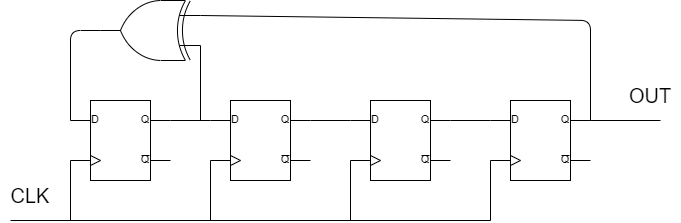
\includegraphics[width=1\linewidth]{Bilder/LFSR.drawio.png}
\caption{LFSR}
\label{fig:LFSR}
\end{figure}

\subsection{Aktivt filter topologi}
\label{aktivtFilter}

Aktive filtre benytter seg av kondensatorer og operasjonsforsterkere for å filtrere bort uønskede frekvenser. Utifra hvilken kretstopologi man velger får man forskjellige type filter og i dette designet skal vi se på Delyiannis-Friend topologien for å lage et andreordens båndpass filter. Delyiannis - Friend topologien er kan konfigureres ved å endre impedansen til hver av komponentene $Z_1 ... Z_5$ til filteret som vist i figur \ref{fig:SallenKey}\cite{Active Filter}. 

\begin{figure} [!h]
\centering
\includegraphics[width=0.7\linewidth]{Bilder/Båndpass.drawio.png}
\caption{Delyiannis - Friend-topologi}
\label{fig:SallenKey}
\end{figure}
\newpage
Verdiene til de ulike komponentene kan bestemmes ut i fra følgene ligninger \cite{Active Filter}:
%f_0
\begin{equation}
    \label{eq:f}
    f_0 = \frac{1}{2 \pi C \sqrt{(R_1||R_2)R_3}}
\end{equation}
%H
\begin{equation}
    \label{eq:h}
    H_0 = \frac{R_3}{2R_1}
\end{equation}
%Q
\begin{equation}
    \label{eq:q}
    Q = \frac{f_0}{B} = \frac{1}{2} \sqrt{\frac{R_3}{R_1||R_2}}
\end{equation}
%R1
\begin{equation}
    \label{eq:r1}
    R_1 = \frac{R_3}{2H_0}
\end{equation}
%R2
\begin{equation}
    \label{eq:r2}
    R_2 = \frac{R_3}{4Q^2 -2H_0}
\end{equation}
%R3
\begin{equation}
    \label{eq:r3}
    R_3 = \frac{Q}{\pi f_0 C}
\end{equation}

En naturlig fremgangsmøte for å bruke ligningene er følgende: \cite{støygenerator}
\begin{enumerate}
    \item Velg en $Q$-faktor.
    \item Velg amplituderesponsen $H_0$ for senterfrekvensen. Ønsker man forsterkning kan maneksperimentere med $H_0$ større enn 1.
    \item Velg kondensatorstørrelse $C$.
    \item Beregn motstanden $R_3$, deretter motstandene $R_2$ og $R_1$.
\end{enumerate}
